\documentclass[14pt]{extbook}
\usepackage{multicol, enumerate, enumitem, hyperref, color, soul, setspace, parskip, fancyhdr} %General Packages
\usepackage{amssymb, amsthm, amsmath, latexsym, units, mathtools} %Math Packages
\everymath{\displaystyle} %All math in Display Style
% Packages with additional options
\usepackage[headsep=0.5cm,headheight=12pt, left=1 in,right= 1 in,top= 1 in,bottom= 1 in]{geometry}
\usepackage[usenames,dvipsnames]{xcolor}
\usepackage{dashrule}  % Package to use the command below to create lines between items
\newcommand{\litem}[1]{\item#1\hspace*{-1cm}\rule{\textwidth}{0.4pt}}
\pagestyle{fancy}
\lhead{Progress Quiz 1}
\chead{}
\rhead{Version B}
\lfoot{3629-3146}
\cfoot{}
\rfoot{Summer C 2021}
\begin{document}

\begin{enumerate}
\litem{
Write the equation of the line in the graph below in Standard Form $Ax+By=C$. Then, choose the intervals that contain $A, B, \text{ and } C$.
\begin{center}
    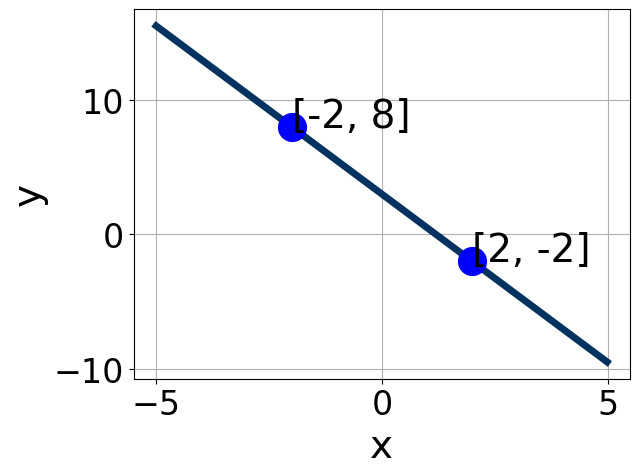
\includegraphics[width=0.5\textwidth]{../Figures/linearGraphToStandardB.png}
\end{center}
\begin{enumerate}[label=\Alph*.]
\item \( A \in [4, 7], \hspace{3mm} B \in [-3.08, -1.52], \text{ and } \hspace{3mm} C \in [-7.9, -5.6] \)
\item \( A \in [-8, 1], \hspace{3mm} B \in [-3.08, -1.52], \text{ and } \hspace{3mm} C \in [-7.9, -5.6] \)
\item \( A \in [-1.5, 4.5], \hspace{3mm} B \in [-0.21, 1.61], \text{ and } \hspace{3mm} C \in [1.6, 5.1] \)
\item \( A \in [4, 7], \hspace{3mm} B \in [1.83, 2.1], \text{ and } \hspace{3mm} C \in [5.1, 9.2] \)
\item \( A \in [-1.5, 4.5], \hspace{3mm} B \in [-1.55, -0.71], \text{ and } \hspace{3mm} C \in [-3.7, -1.5] \)

\end{enumerate} }
\litem{
Find the equation of the line described below. Write the linear equation in the form $ y=mx+b $ and choose the intervals that contain $m$ and $b$.\[ \text{Parallel to } 8 x - 7 y = 13 \text{ and passing through the point } (-7, 7). \]\begin{enumerate}[label=\Alph*.]
\item \( m \in [0.96, 1.48] \hspace*{3mm} b \in [13.02, 14.67] \)
\item \( m \in [-1.2, -0.85] \hspace*{3mm} b \in [-1.17, -0.99] \)
\item \( m \in [0.96, 1.48] \hspace*{3mm} b \in [-15.32, -14.66] \)
\item \( m \in [0.74, 1.11] \hspace*{3mm} b \in [14.79, 15.09] \)
\item \( m \in [0.96, 1.48] \hspace*{3mm} b \in [14.79, 15.09] \)

\end{enumerate} }
\litem{
Solve the linear equation below. Then, choose the interval that contains the solution.\[ \frac{-6x + 7}{2} - \frac{-5x + 7}{6} = \frac{-7x + 3}{8} \]\begin{enumerate}[label=\Alph*.]
\item \( x \in [-0.6, 0.5] \)
\item \( x \in [0.4, 3.3] \)
\item \( x \in [-4.2, -1.8] \)
\item \( x \in [1.6, 4] \)
\item \( \text{There are no real solutions.} \)

\end{enumerate} }
\litem{
Write the equation of the line in the graph below in Standard Form $Ax+By=C$. Then, choose the intervals that contain $A, B, \text{ and } C$.
\begin{center}
    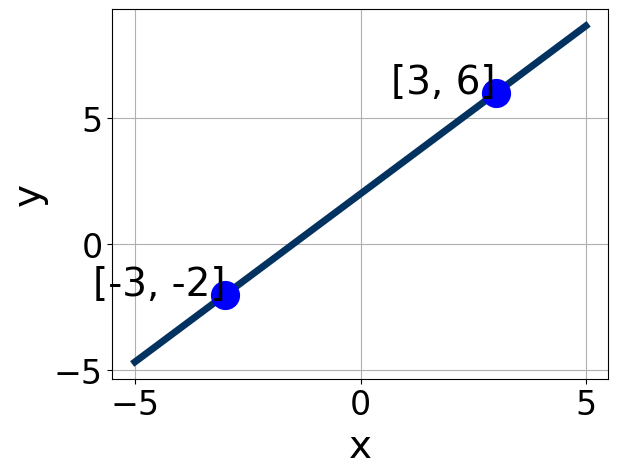
\includegraphics[width=0.5\textwidth]{../Figures/linearGraphToStandardCopyB.png}
\end{center}
\begin{enumerate}[label=\Alph*.]
\item \( A \in [-2.1, -1.2], \hspace{3mm} B \in [-2.7, -0.4], \text{ and } \hspace{3mm} C \in [-2.1, -0.5] \)
\item \( A \in [2.6, 7.1], \hspace{3mm} B \in [2.5, 5.2], \text{ and } \hspace{3mm} C \in [4.8, 9.5] \)
\item \( A \in [-2.1, -1.2], \hspace{3mm} B \in [0.5, 1.4], \text{ and } \hspace{3mm} C \in [-0.1, 2.9] \)
\item \( A \in [2.6, 7.1], \hspace{3mm} B \in [-3.2, -2.6], \text{ and } \hspace{3mm} C \in [-7.8, -4] \)
\item \( A \in [-4.9, -3.5], \hspace{3mm} B \in [2.5, 5.2], \text{ and } \hspace{3mm} C \in [4.8, 9.5] \)

\end{enumerate} }
\litem{
Find the equation of the line described below. Write the linear equation in the form $ y=mx+b $ and choose the intervals that contain $m$ and $b$.\[ \text{Parallel to } 7 x - 5 y = 7 \text{ and passing through the point } (7, -4). \]\begin{enumerate}[label=\Alph*.]
\item \( m \in [0.83, 2.03] \hspace*{3mm} b \in [12.9, 16.6] \)
\item \( m \in [-2.1, -1.18] \hspace*{3mm} b \in [5.4, 7.1] \)
\item \( m \in [0.59, 0.78] \hspace*{3mm} b \in [-15.3, -13.5] \)
\item \( m \in [0.83, 2.03] \hspace*{3mm} b \in [-15.3, -13.5] \)
\item \( m \in [0.83, 2.03] \hspace*{3mm} b \in [-11.2, -10.6] \)

\end{enumerate} }
\litem{
Solve the linear equation below. Then, choose the interval that contains the solution.\[ \frac{3x + 4}{3} - \frac{-7x -7}{5} = \frac{5x -9}{2} \]\begin{enumerate}[label=\Alph*.]
\item \( x \in [44.33, 46.33] \)
\item \( x \in [-4.45, -0.45] \)
\item \( x \in [67.33, 78.33] \)
\item \( x \in [197, 204] \)
\item \( \text{There are no real solutions.} \)

\end{enumerate} }
\litem{
First, find the equation of the line containing the two points below. Then, write the equation in the form $ y=mx+b $ and choose the intervals that contain $m$ and $b$.\[ (-2, -10) \text{ and } (-9, 11) \]\begin{enumerate}[label=\Alph*.]
\item \( m \in [2, 12] \hspace*{3mm} b \in [33, 41] \)
\item \( m \in [-6, -2] \hspace*{3mm} b \in [10, 17] \)
\item \( m \in [-6, -2] \hspace*{3mm} b \in [-20, -9] \)
\item \( m \in [-6, -2] \hspace*{3mm} b \in [-8, -6] \)
\item \( m \in [-6, -2] \hspace*{3mm} b \in [19, 23] \)

\end{enumerate} }
\litem{
Solve the equation below. Then, choose the interval that contains the solution.\[ -2(-8x + 12) = -5(-18x -16) \]\begin{enumerate}[label=\Alph*.]
\item \( x \in [-1.56, -1.34] \)
\item \( x \in [-1.1, -0.59] \)
\item \( x \in [0.61, 1.06] \)
\item \( x \in [-0.75, -0.25] \)
\item \( \text{There are no real solutions.} \)

\end{enumerate} }
\litem{
First, find the equation of the line containing the two points below. Then, write the equation in the form $ y=mx+b $ and choose the intervals that contain $m$ and $b$.\[ (7, -6) \text{ and } (10, -5) \]\begin{enumerate}[label=\Alph*.]
\item \( m \in [0.19, 0.59] \hspace*{3mm} b \in [-9.5, -7.3] \)
\item \( m \in [0.19, 0.59] \hspace*{3mm} b \in [-14.2, -12.1] \)
\item \( m \in [0.19, 0.59] \hspace*{3mm} b \in [6.3, 9.3] \)
\item \( m \in [0.19, 0.59] \hspace*{3mm} b \in [-16.5, -13.7] \)
\item \( m \in [-0.48, -0.14] \hspace*{3mm} b \in [-3, -0.1] \)

\end{enumerate} }
\litem{
Solve the equation below. Then, choose the interval that contains the solution.\[ -5(12x + 6) = -2(3x + 11) \]\begin{enumerate}[label=\Alph*.]
\item \( x \in [-0.22, 0] \)
\item \( x \in [-1.08, -0.8] \)
\item \( x \in [0.85, 1.13] \)
\item \( x \in [-0.81, -0.78] \)
\item \( \text{There are no real solutions.} \)

\end{enumerate} }
\end{enumerate}

\end{document}